\documentclass[11pt,english]{article}
\usepackage[a4paper,bindingoffset=0.1in,%
            left=0.5in,right=0.5in,top=0.5in,bottom=0.5in,%
            footskip=.25in]{geometry}
\usepackage[utf8]{inputenc}
\usepackage{graphicx}
\usepackage{hyperref}
\begin{document}
\title{Speech Command Model}
\author{Pradeep Moturi (es16btech11016)}
\date{May 2020}

\sloppy
\maketitle
\setlength{\columnsep}{0.25in}
\twocolumn
\tableofcontents

\section{Introduction}
This is the report of my work done under Dr. G V V Sharma on building a speech command recognition model for a voice bot. 
The model used is based on concepts of Convolution, LSTM and Attention and is derived from \cite{Paper}.

\section{Create Data}
\begin{enumerate}
    \item Set 16KHz as sampling rate
    \item Record 80 utterances of each command.
    \item Trim each utterance to one second.
    \item Save samples of each command in different folders\\
        Dataset/forward\\
        Dataset/back\\
        Dataset/left\\
        Dataset/right\\
        Dataset/stop
\end{enumerate}
Used Audacity to do this.

\section{Loading Data}
I've used soundfile package to read the .wav. You may choose to use any other package like wavefile, librosa etc to do the same job.\\
As this is one of the slowest part, I've stored the loaded data as a numpy file for ease and speed of access. Now, I can load the data from npy file if repeating the experiment.

\section{Split dataset}
Do a stratified split of the dataset into train and test set with 20\% as test samples.\\
Set a random seed for reproducing the split.

\section{Augment data}
Augment each audio sample by time shifting in 25000 length vectors filled with zeros. \\
Take steps of 500 to create 18 files per sample

\section{Feature Extraction}
MFCCs are most prominent features used in audio processing.
Normalizing the MFCCs over the frequency axis is found to reduce effect of noise.\\
Kapre is a python package that provides layers for audio processing that are compatible with keras and utilize GPU for faster processing. Kapre provides us with a layer basically\\

\textit{Melspectrogram (padding='same', sr=16000, n\_mels=39, n\_dft = 1024, power\_melgram=2.0, return\_decibel\_melgram=True, trainable\_fb=False, trainable\_kernel=False,  name='mel\_stft')}\\

\textbf{Arguments to the layer}\\
\textbf{padding:} Padding when convoluting\\
\textbf{sr:} Sampling rate of audio provided\\
\textbf{n\_mels:} number of coefficients to return\\
\textbf{n\_dft:} width \\
\textbf{power\_melgram:} exponent to raise log-mel-amplitudes before taking DCT. Using power 2 is shown to increase performance by reducing effect of noise\\
\textbf{return\_decibel\_melgram:} If to return log over values\\
\textbf{trainable\_fb:} If filter bank trainable\\
\textbf{trainable\_kernel:} If the kernel is trainable

\section{Building Model}
\subsection{Concept}
\begin{enumerate}
    \item Using Convolutional layers ahead of LSTM is shown to improve performance in several research papers.
    \item BatchNormalization layers are added to improve convergence rate.
    \item Using Bidirectional LSTM is optimal when complete input is available. But this increases the runtime two-fold.
    \item Final output sequence of LSTM layer is used to calculate importance of units in LSTM using a FC layer.
    \item Then take the dot product of unit importance and output sequences of LSTM to get Attention scores of each time step.
    \item Take the dot product of Attention scores and the output sequences of LSTM to get attention vector.
    \item Add an additional FC Layer and then to output Layer with SoftMax Activation.
\end{enumerate}

\subsection{Hyper parameters}
\begin{itemize}
    \item \textbf{sparse\_categorical\_crossentropy} is used as \textbf{Loss} because only output which should be 1 is given instead of One Hot Encoding.
    \item \textbf{sparse\_categorical\_accuracy} is used as performance \textbf{Metric} for the above reason.
    \item \textbf{Adam} is used as \textbf{Optimizer}. Adam is adaptive learning rate optimization algorithm. This is shown to achieve a faster convergence because of having all the features of other optimization algorithms.
    \item Batch size of 15 is used
\end{itemize}

\subsection{Notations}
\textbf{Operators:}
\begin{itemize}
    \item $\times$ indicate matrix multiplication
    \item $*$ denote convolution (0 padding to same size)
    \item . denote dot product
    \item +,- can expand dimensions of their arguments
\end{itemize}
\vspace{0.25em}
\textbf{Format:}\\ 
Layer Name ( Layer Type ) (Output Size). \\
\textbf{Parameters}\\
\textbf{Equations}\\
\textbf{Output}\\
= $equation$\\
\\
Layer name indicates output of the corresponding layer.\\
Let us understand the maths behind the model.

\subsection{Math}
You can have a overall look at the architecture of the model in Fig [\ref{fig: Architecture}]. Lets observe the math in each layer below.
\begin{enumerate}
    \setcounter{enumi}{-1}
    \item Input (InputLayer) (49, 39, 1)
    
    \item Conv1 (Conv2D)                    (49, 39, 10)\\
    \textbf{Parameters:} \\
    Kernel = (5, 1, 1, 10),  Bias = (10)\\
    \textbf{Conv1[:,:,i]} \\
    = $Kernel[:,:,:,i] * Input + Bias[i]$
    
    \item BN1 (BatchNormalization)          (49, 39, 10)\\
    \textbf{Parameters:} \\
    Trainable: $\gamma$ = (10), $\beta$ = (10), \\
    Non-Trainable: Mean = (10), Std = (10)\\
    \textbf{Equations:} \\
    Mean[i] = $mean(Conv1[:,:,i])$\\
    Std[i] = $std(Conv1[:,:,i])$\\
    \textbf{BN1[i]} \\
    = $(Conv1[:,:,i]-Mean[i]) \frac{\gamma[i]}{Std[i]} + \beta[i]$
                  
    \item Conv2 (Conv2D)                    (49, 39, 1)\\
    \textbf{Parameters:} \\
    Kernel = (5, 1, 10, 1),  Bias = (1)\\
    \textbf{Conv2[:,:,1]}\\ 
    = $Kernel[:,:,:,1] * BN1 + Bias$
                  
    \item BN2 (BatchNormalization)          (49, 39, 1)\\
    \textbf{Parameters:} \\
    Trainable: $\gamma$ = (1), $\beta$ = (1), \\
    Non-Trainable: Mean = (1), Std = (1)\\
    \textbf{Equations:} \\
    Mean[i] = $mean(Conv2[:,:,i])$\\
    Std[i] = $std(Conv2[:,:,i])$\\
    \textbf{BN2[i]} \\
    = $(Conv2[:,:,i]-Mean[i]) \frac{\gamma[i]}{Std[i]} + \beta[i]$
    
    \item Squeeze (Reshape)                 (49, 39)\\
    \textbf{Squeeze} \\
    = $BN2.reshape(49,39)$
    
    \item LSTM\_Sequences (LSTM)            (49, 64)\\
    \textbf{Parameters:} \\
    $U^i = U^f = U^o = U^g = (39,64),\\
    W^i = W^f = W^o = W^g = (64,64),\\
    B^i = B^f = B^o = B^g = (64) \\$
    \textbf{Equations:} \\
    $i_t = \sigma(Squeeze[:,t]\times U^i + h_{t-1}\times W^i + B^i) \\
    f_t = \sigma(Squeeze[:,t]\times U^f + h_{t-1}\times W^f + B^f) \\
    o_t = \sigma(Squeeze[:,t]\times U^o + h_{t-1}\times W^o + B^o) \\
    \widetilde{C}_t = tanh(Squeeze[:,t]\times U^g + h_{t-1}\times W^g + B^g) \\
    C_t = \sigma(f_t*C_{t-1} + i_t*\widetilde{C}_t) \\
    h_t = tanh(C_t)*o_t
    \\
    \textbf{LSTM\_Sequences[t]}\\
    = h_t$
    
    \item FinalSequence (Lambda)            (64)\\
    \textbf{FinalSequence}\\
    = $LSTM\_Sequences[-1,:]$
    
    \item UnitImportance (Dense)            (64)\\
    \textbf{Parameters:} \\
    Weights = (64,64), Bias = (64)\\
    \textbf{UnitImportance} \\
    = $Weights \times FinalSequence + Bias$
         
    \item AttentionScores (Dot)             (49)\\
    \textbf{AttentionScores[i]} \\
    = $UnitImportance . LSTM\_Sequences[i,:]$
      
    \item AttentionSoftmax (Softmax)        (49)\\
    \textbf{AttentionSoftmax[i]} \\
    =$\frac{exp(AttentionScores[i])}{\sum_j exp(AttentionScores[j])}$
    
    \item AttentionVector (Dot)             (64)\\
    \textbf{AttentionVector[i]} \\
    = $AttentionSoftmax . LSTM\_Sequences[:,i]$
    
    \item FC (Dense)                        (32)\\
    \textbf{Parameters:} \\
    Weights = (64,64), Bias = (64)\\     
    \textbf{FC}\\ 
    = $Weights \times AttentionVector + Bias$
    
    \item Output (Dense)                    (5)\\
    \textbf{Parameters:} \\
    Weights = (32,5), Bias = (5)\\
    \textbf{Output} \\
    = $SoftMax(Weights \times FC + Bias)$
    
\end{enumerate}    
After an input passes through the layers, the training happens by principle of Back Propagating Loss or Gradients calculated by Sparse Categorical Cross-Entropy and updating weights using the Adam Optimizer update equations.   

\section{Training}

\subsection{Back Propagation}
Back propagation is the algorithm used to calculate the gradient of loss w.r.t all the parameters in the neural network. Gradient of Loss w.r.t parameter is the direction in which the parameter should move such that decrease in loss will be maximum. This algorithm uses the property of differentiation called chain rule. This algorithm is based on dynamic programming hence removes any redundant calculations of intermediate gradients.\\
Each layer and function is programmed to calculate the gradient of loss w.r.t it's trainable parameters and input given the input and gradient of loss w.r.t its output.\\
Gradient of loss w.r.t input of the current layer or function is back propagated as gradient of loss w.r.t output of previous layer or function. Hence, the name back propagation.

\subsection{Adam Optimizer}
Back propagation calculates the gradient of loss w.r.t each parameter. But a adaptive learning rate algorithm will be used to update the weights in a more calculated manner.\\
Unlike SGD, Adam maintains few training parameters independently for each network parameter while SGD only has a single learning rate parameter for all the weights of the network. Adam is a combination of AdaGrad and RMSProp (Two other optimization algorithms).\\
RMSProp uses only Average first moment (running average of the gradient) while Adam also uses Average second moment (running average of the square of gradient ) in the learning rate calculation.\\
For each network parameter, Adam maintains 
\begin{itemize}
    \item \textbf{Alpha}
    Also referred to as the learning rate or step size. 
    Proportion of the update to be added to the weight.
    \item \textbf{Beta1}
    The exponential decay rate for the first moment estimates (e.g. 0.9).
    \item \textbf{Beta2}
    The exponential decay rate for the second-moment estimates (e.g. 0.999)
    \item \textbf{Epsilon}
    Is a very small number to prevent any division by zero in the implementation (e.g. 10E-8)
\end{itemize}


\begin{figure}[!ht]
\centering
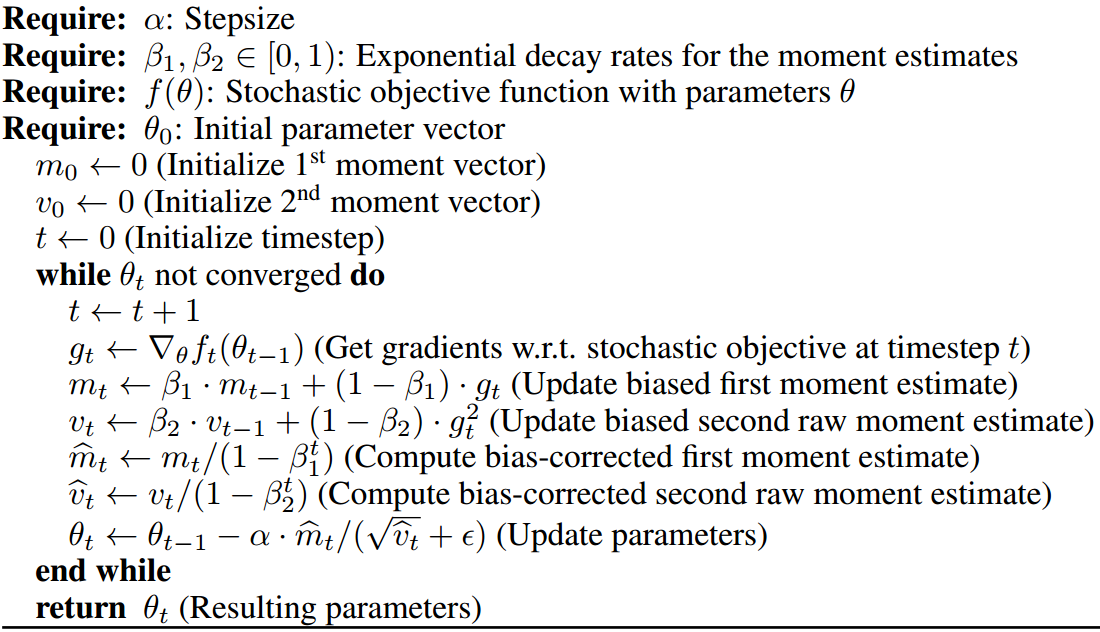
\includegraphics[width=\columnwidth]{./Figs/Adam.eps}
\caption{ Adam algorithm}.
\label{fig: Adam}	
\end{figure}


\section{Testing}
\begin{enumerate}
    \item Augment the test set same as training set.
    \item Extract MFCCs using same method as training set
    \item Test set is passed as validation set to fit method of model.
    \item The performance of model on test set is calculated after every epoch.
\end{enumerate}

\section{Visualize Attention}
\begin{enumerate}
    \item Now build a sub model from the trained model. Take same input layer but add ‘AttentionSoftmax’ layer as additional output layer.
    \item Pass MFCCs of test samples to predict method.
    \item Now plot log of Attention Scores and corresponding input vector before taking MFCCs on different axes.
    \item By looking at Fig [\ref{fig: Attention}] and Fig [\ref{fig: Sample}], We observe that Attention Scores are high on informative part.
    \begin{figure}[!ht]
    \centering
    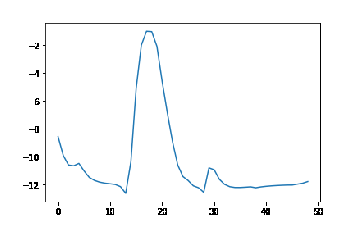
\includegraphics[width=\columnwidth]{./Figs/Attention.eps}
    \caption{ log(Attention Scores)}.
    \label{fig: Attention}	
    \end{figure}
    \begin{figure}[!ht]
    \centering
    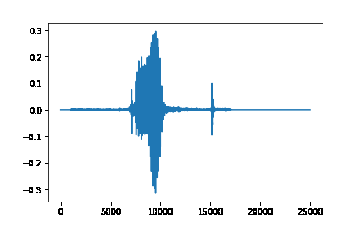
\includegraphics[width=\columnwidth]{./Figs/Sample.eps}
    \caption{ Raw sample}.
    \label{fig: Sample}	
    \end{figure}
    
\end{enumerate}

 
\section{Observations}
\begin{itemize}
    \item Smaller batch size is prefferable
    \item Setting power\_melgram=2 of Melspectogram gave faster convergence.
\end{itemize}
\section{Files}
\begin{itemize}
    \item Src/DataGenerator.py: Augments the data
    \item Src/FeatureExtractor.py: Extracts MFCC coefficients
    \item Src/TrainModel.py: Trains model and saves it in h5 file
    \item ColabNotebook.ipynb: Use this for experimental purpose
\end{itemize}

\section{Further}
\begin{itemize}
    \item Different augmentation techniques like adding noise, changing pitch, speed etc.
    \item Given the low complexity of our dataset, We can replace LSTM with GRU which is little less complex but shown to outperform LSTM in many scenarios. 
    \item We can tune the arguments to Melspectrogram 
    \item Changing the model architecture like layers and units in layers.
    \item Further the scope of project to check performance on Google’s Speech Command Datasets (v1 and v2) and participate in Kaggle challenge by google
[https://www.kaggle.com/c/tensorflow-speech-recognition-challenge/]

\end{itemize}

\begin{thebibliography}{9}
\bibitem{Paper} 
Douglas Coimbra de Andrade, Sabato Leo, Martin Loesener Da Silva Viana, Christoph Bernkopf. 
\textit{A neural attention model for speech command recognition}. 

\end{thebibliography}
%%
\begin{figure}[!ht]
\centering
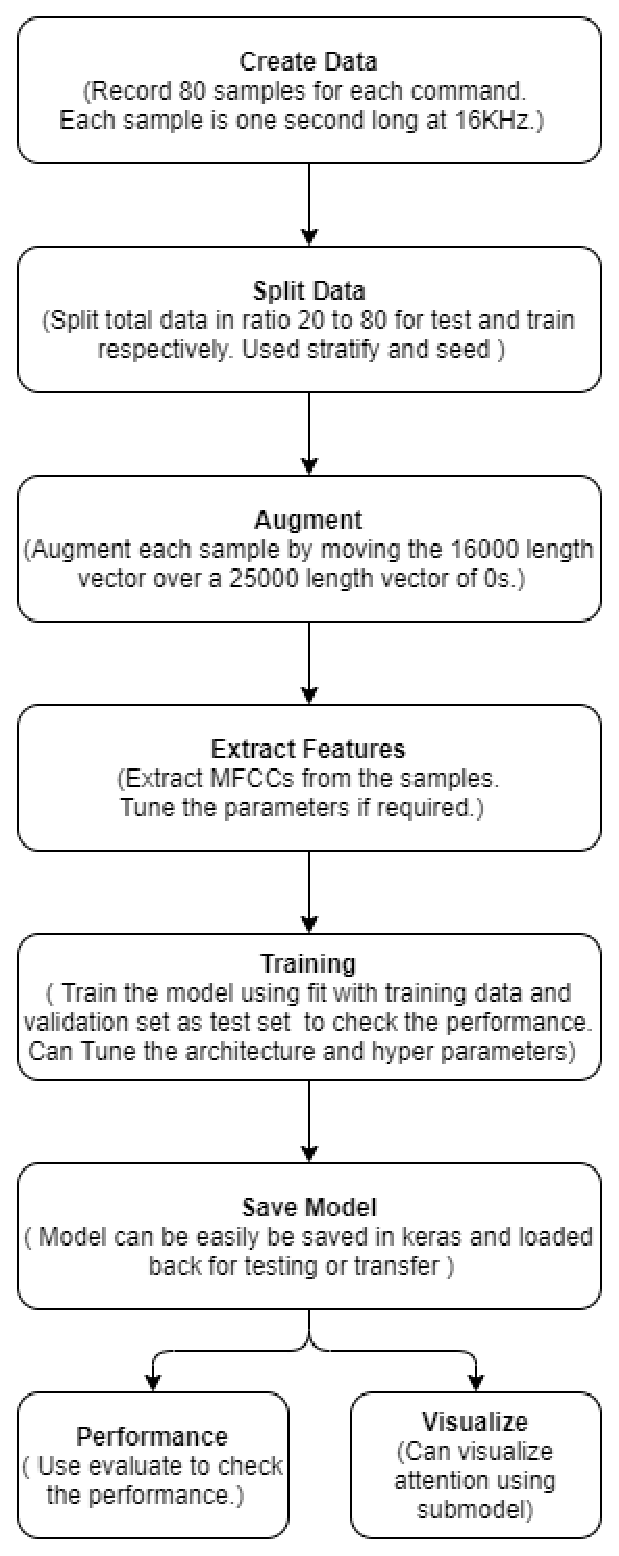
\includegraphics[width=\columnwidth]{./Figs/Flow.eps}
\caption{ Data Flow Diagram}.
\label{fig: Flow}	
\end{figure}
%
\begin{figure}[!ht]
\centering
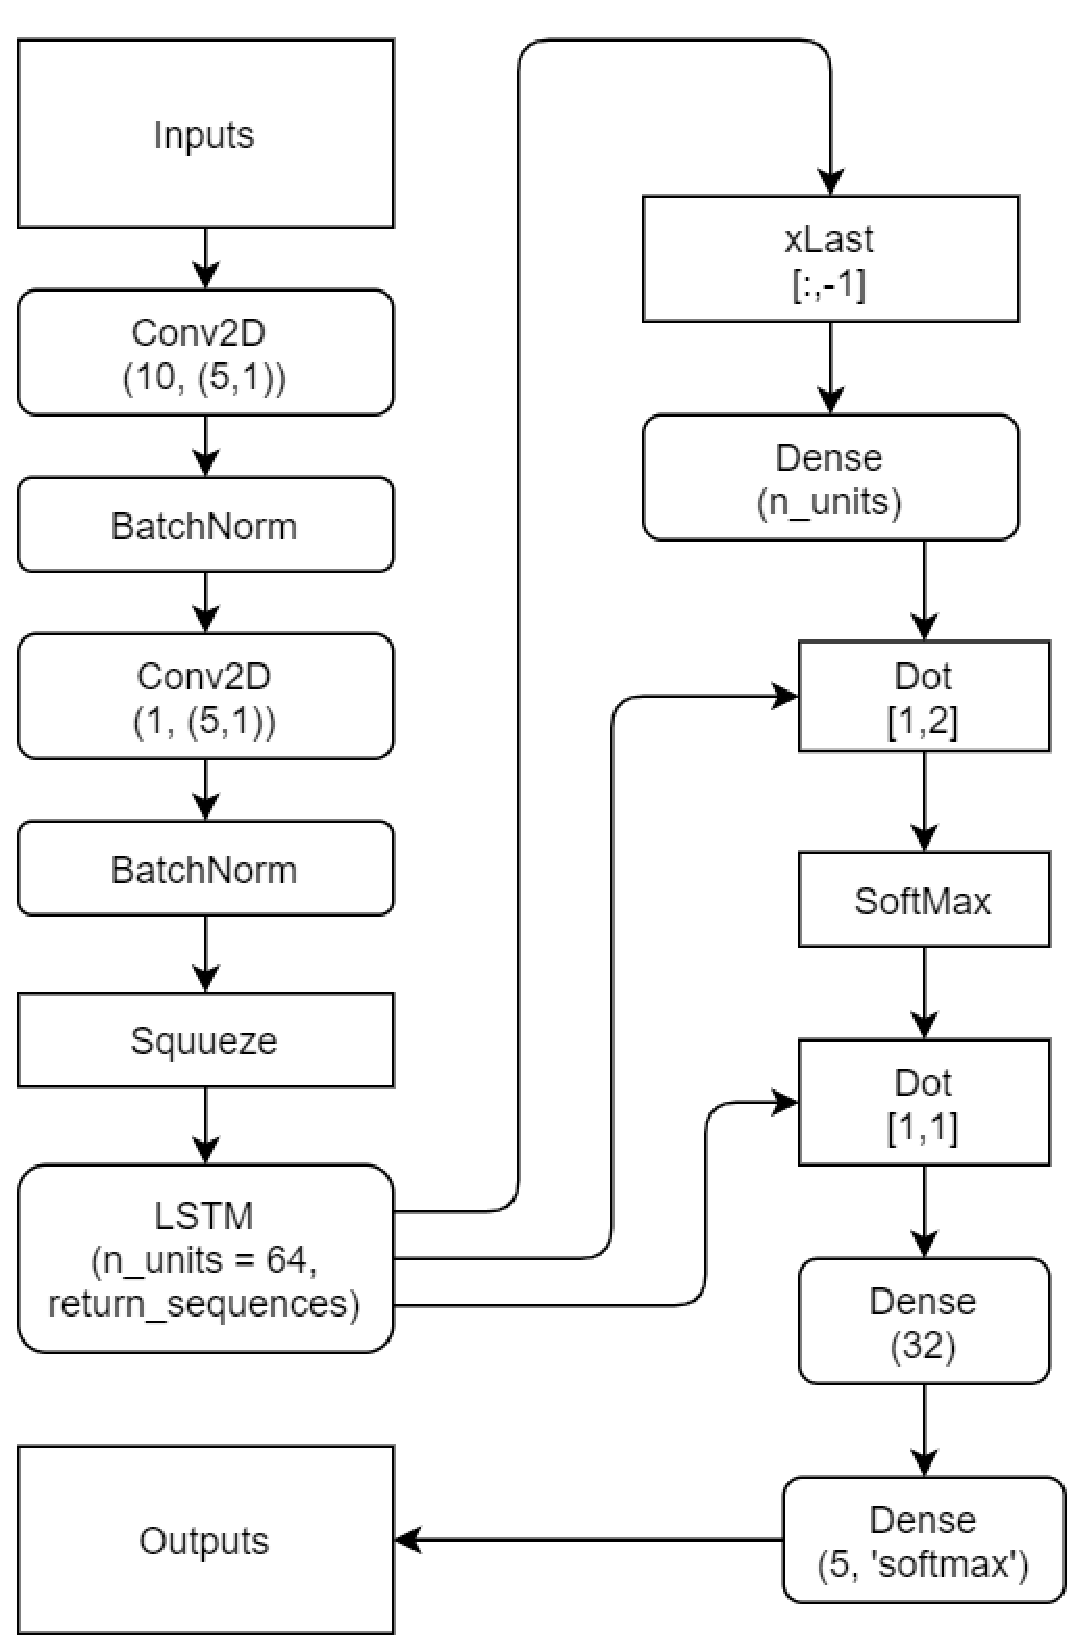
\includegraphics[width=\columnwidth]{./Figs/Model.eps}
\caption{ Model Diagram}.
\label{fig: Model}	
\end{figure}

\onecolumn

\begin{figure}[!ht]
\centering
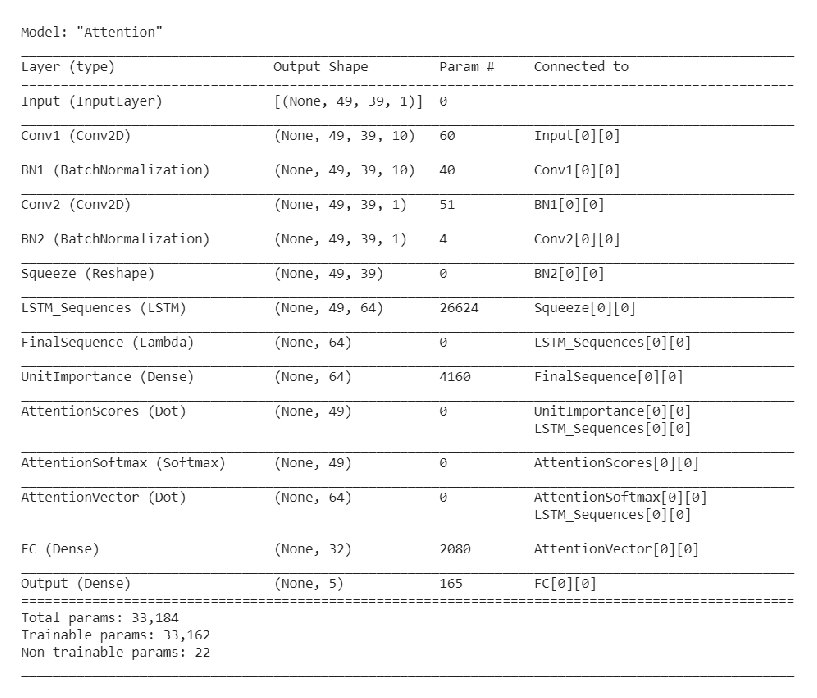
\includegraphics[width=\columnwidth]{./Figs/Architecture.eps}
\caption{ Model Architecture}.
\label{fig: Architecture}	
\end{figure}


\end{document}
